\chapter{Arbeitsgrundlagen}
% ==================================================================
\setcounter{page}{1} \thispagestyle{fancy} 
% ==================================================================
\section{Das Röntgen-Spektrum}
Wenn schnelle Elektronen auf Materie treffen, dann entstehen Röntgenstrahlen. Eine Röntgen-Röhre besteht aus (siehe Abbildung \ref{fig:roentgen_roehre}):
\begin{itemize}
\item[\textbf{K}] \textbf{Glühkathode}
\item[\textbf{A}] \textbf{massive Anode} (je nach Verwendungszweck ein Metall mittlerer bis hoher Ordnungszahl)
\item[\textbf{U}] \textbf{Hochspannung} (Bereich von $10kV$ bis zu einigen $100kV$)
\end{itemize}
Die Glühkathode und die massive Anode sind dabei von einem evakuierten Glaskolben umschlossen. Von der Kathode emittieren Elektronen, welche von der angelegten Hochspannung beschleunigt werden. Mit einer fokussierten Energie von ungefähr $E_{k} = e*U$ prallen diese dann auf die Anode. In einer Schicht von wenigen $\mu m$ Dicke verlieren die Elektronen ihre Energie durch eine Kette von Stoßprozessen. Hauptsächlich durch Anregung und Ionisation der Metallatome ($>99\%$). Diese Energie wird in Wärme umgewandelt, weshalb die Anoden rotiert oder mit Wasser gekühlt werden müssen. Somit bleibt nur noch ein kleiner Rest übrig ($<1\%$), welcher in Röntgenstrahlung umgesetzt wird. Die resultierende Strahlung entspricht einer isotropen Strahlung (\textit{Isotropie}\footnote{\textit{kursiv} geschriebene Begriffe sind im Kapitel \nameref{chap:begriffsexplikation} genauer erläutert}), was eine Abschirmung erfordert. Die Nutzstrahlung wird mit einem Bleikollimator ausgeblendet. Die Anode ist abgeschrägt und der Kolben mit einem Fenster aus dünnerem Glas oder Beryllium versehen, damit die Absorptionen  niedrig gehalten werden können.
\begin{figure}[h]
\centering
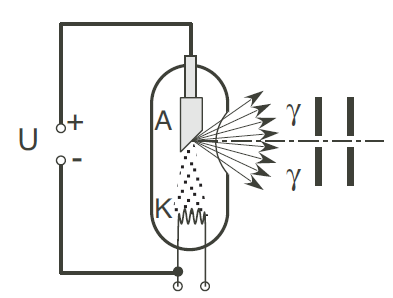
\includegraphics[scale=1.5]{Bilder/roentgen_roehre.png} 
\label{fig:roentgen_roehre}
\caption{Röntgen-Röhre}
\end{figure}
\newpage

\begin{wrapfigure}{r}{0.5\textwidth}
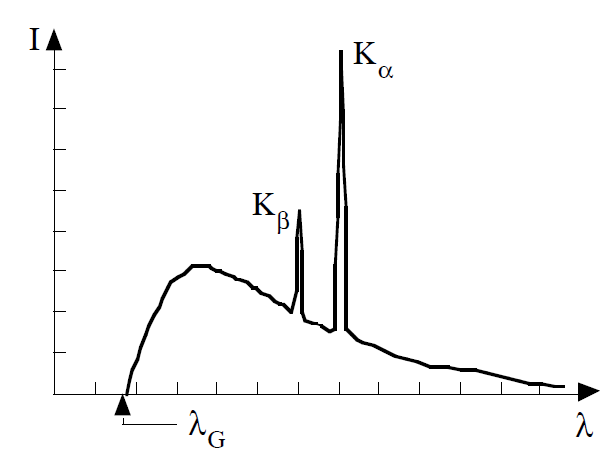
\includegraphics[width=0.48\textwidth]{Bilder/roentgen_spektrum.png}
\caption[Röntgenspektrum]{Röntgenspektrum: \textbf{I} steht für die Intensität und $\lambda$ für die Wellenlänge.}
\vspace{-1.5cm}
\label{fig:roentgenspektrum}
\end{wrapfigure}
Aus der Abbildung \ref{fig:roentgenspektrum} kann entnommen werden, dass das Röntgenspektrum aus zwei Komponenten besteht:
\begin{itemize}
\item \textbf{Bremskontinuum}: Es weisst eine unspezifische Form auf und beginnt am kurzweiligen Ende bei einem von der angelegten Spannung abhängigen Punkt ($\lambda_{G}$)
\item \textbf{Röntgenlinien}: ($K_{\alpha}$ \& $K_{\beta}$) Diese sind charakteristisch für das Anodenmaterial und hängen nicht von der Spannung ab
\end{itemize}

\subsection{Die Bremsstrahlung}
\blindtext